

% \chapter{Functions  |  函数}
\chapter{函数}
\label{funcchap}

%🍁% In the context of programming, a {\bf function} is a named sequence of
%🍁% statements that performs a computation.  When you define a function,
%🍁% you specify the name and the sequence of statements.  Later, you can
%🍁% ``call'' the function by name.
%🍁% \index{function}

在编程的语境下,{\em 函数} (function)  是指一个有命名的、执行某个计算的语句序列(sequence of statements) 。  在定义一个函数的时候,你需要指定函数的名字和语句序列。  之后,你可以通过这个名字``{\em 调用} (call)''该函数。
\index{function}  \index{函数}

%
%%
% \section{Function calls  |  函数调用}
\section{函数调用}
\label{functionchap}
\index{function call}
\index{函数调用}

%🍁% We have already seen one example of a {\bf function call}:

我们已经看见过了 {\em 函数调用} (function call) 的例子。

\begin{lstlisting}
>>> type(42)
<class 'int'>
\end{lstlisting}

%
%🍁% The name of the function is {\tt type}.  The expression in parentheses
%🍁% is called the {\bf argument} of the function.  The result, for this
%🍁% function, is the type of the argument.

这个函数的名字是 ``type''。 括号中的表达式被称为这个函数的 {\em 实参} (argument)。 这个函数执行的结果,就是实参的类型。
\index{parentheses!argument in}
\index{括号!实参}

%🍁% It is common to say that a function ``takes'' an argument and ``returns''
%🍁% a result.  The result is also called the {\bf return value}.

人们常说函数``接受 (accept)''实参,然后 ``返回 (return)''一个结果。
该结果也被称为 {\em 返回值} (return value)。
\index{argument}  \index{return value}
\index{实参}  \index{返回值}

%🍁% Python provides functions that convert values
%🍁% from one type to another.  The {\tt int} function takes any value and
%🍁% converts it to an integer, if it can, or complains otherwise:

Python提供了能够将值从一种类型转换为另一种类型的内建函数。
函数 \li{int} 接受任意值,并在其能做到的情况下,将该值转换成一个整型数,
否则会报错:
\index{conversion!type}  \index{type conversion}
\index{int function}  \index{function!int}
\index{转换!类型}  \index{类型转换}
\index{整数型函数}  \index{函数!整数型}

\begin{lstlisting}
>>> int('32')
32
>>> int('Hello')
ValueError: invalid literal for int(): Hello
\end{lstlisting}

%
%🍁% {\tt int} can convert floating-point values to integers, but it
%🍁% doesn't round off; it chops off the fraction part:

\li{int} 能将浮点数转换为整型数,但是它并不进行舍入;只是截掉了小数点部分:

\begin{lstlisting}
>>> int(3.99999)
3
>>> int(-2.3)
-2
\end{lstlisting}

%
%🍁% {\tt float} converts integers and strings to floating-point
%🍁% numbers:

\li{float} 可以将整型数和字符串转换为浮点数:
\index{float function}  \index{function!float}
\index{浮点型函数}  \index{函数!浮点型}

\begin{lstlisting}
>>> float(32)
32.0
>>> float('3.14159')
3.14159
\end{lstlisting}

%
%🍁% Finally, {\tt str} converts its argument to a string:

\li{str} 可以将其实参转换成字符串:
\index{str function}  \index{function!str}
\index{字符串函数}  \index{函数!字符串}

\begin{lstlisting}
>>> str(32)
'32'
>>> str(3.14159)
'3.14159'
\end{lstlisting}

%
%%
% \section{Math functions  |  数学函数}
\section{数学函数}
\index{math function}  \index{function, math}
\index{数学函数}  \index{函数, 数学}


%🍁% Python has a math module that provides most of the familiar
%🍁% mathematical functions.  A {\bf module} is a file that contains a
%🍁% collection of related functions.

Python中有一个数学函数模块,提供了大部分常用的数学函数。
{\em 模块} (module) 是指一个包含相关函数集合的文件。
\index{module}  \index{module object}
\index{模块}  \index{模块对象}

%🍁% Before we can use the functions in a module, we have to import it with
%🍁% an {\bf import statement}:

在使用模块之前,我们需要通过 {\em 导入语句} (import statement) 导入该模块:

\begin{lstlisting}
>>> import math
\end{lstlisting}

%
%🍁% This statement creates a {\bf module object} named math.  If
%🍁% you display the module object, you get some information about it:

这条语句会生成一个名为 ``math'' 的 {\em 模块对象} (module object) 。
如果你打印这个模块对象,你将获得关于它的一些信息:


\begin{lstlisting}
>>> math
<module 'math' (built-in)>
\end{lstlisting}

%
%🍁% The module object contains the functions and variables defined in the
%🍁% module.  To access one of the functions, you have to specify the name
%🍁% of the module and the name of the function, separated by a dot (also
%🍁% known as a period).  This format is called {\bf dot notation}.

该模块对象包括了定义在模块内的所有函数和变量。
想要访问其中的一个函数,你必须指定该模块的名字以及函数名,
并以点号(也被叫做句号)分隔开来。 这种形式被称作 {\em 点标记法} (dot
notation)。
\index{dot notation}  \index{点标记法}

\begin{lstlisting}
>>> ratio = signal_power / noise_power
>>> decibels = 10 * math.log10(ratio)

>>> radians = 0.7
>>> height = math.sin(radians)
\end{lstlisting}

%
%🍁% The first example uses \verb"math.log10" to compute
%🍁% a signal-to-noise ratio in decibels (assuming that \verb"signal_power" and
%🍁% \verb"noise_power" are defined).  The math module also provides {\tt log},
%🍁% which computes logarithms base {\tt e}.

第一个例子使用\li{math.log10} 计算分贝信噪比(假设 \li{signal_power}  和\li{noise_power} 已经被定义了)。
math 模块也提供了 \li{log} 函数,用于计算以 $e$ 为底的对数。
\index{log function}  \index{function!log}  \index{sine function}
\index{radian}  \index{trigonometric function}  \index{function, trigonometric}

%🍁% The second example finds the sine of {\tt radians}.  The name of the
%🍁% variable is a hint that {\tt sin} and the other trigonometric
%🍁% functions ({\tt cos}, {\tt tan}, etc.)  take arguments in radians. To
%🍁% convert from degrees to radians, divide by 180 and multiply by
%🍁% $\pi$:

第二个例子计算 \li{radians} 的正弦值。
变量名暗示了 \li{sin} 及其它三角函数( \li{cos}、\li{tan} 等)接受弧度(radians)实参。 度数转换为弧度,需要除以$180$,并乘以 $\pi$ :


\begin{lstlisting}
>>> degrees = 45
>>> radians = degrees / 180.0 * math.pi
>>> math.sin(radians)
0.707106781187
\end{lstlisting}

%
%🍁% The expression {\tt math.pi} gets the variable {\tt pi} from the math
%🍁% module.  Its value is a floating-point approximation
%🍁% of $\pi$, accurate to about 15 digits.

表达式 \li{math.pi} 从 \li{math} 模块中获得变量 \li{pi} 。
该变量的值是 $\pi$ 的一个浮点数近似值,精确到大约15位数。
\index{pi}  \index{$\pi$}
\index{圆周率}

%🍁% If you know trigonometry, you can check the previous result by comparing it to the square root of two divided by two:

如果你了解懂几何学 (trigonometry) ,你可以将之前的结果和二分之根号二进行比较,检查是否正确:
\index{sqrt function}  \index{function!sqrt}

\begin{lstlisting}
>>> math.sqrt(2) / 2.0
0.707106781187
\end{lstlisting}
%

%
%%
% \section{Composition  |  构建}
\section{构建}
\index{composition}

%🍁% So far, we have looked at the elements of a program---variables,
%🍁% expressions, and statements---in isolation, without talking about how to
%🍁% combine them.

目前为止,我们已经分别介绍了程序的基本元素 --- 变量、表达式和语句,但是还没有讨论如何将它们组合在一起。

%🍁% One of the most useful features of programming languages is their
%🍁% ability to take small building blocks and {\bf compose} them.  For
%🍁% example, the argument of a function can be any kind of expression,
%🍁% including arithmetic operators:

编程语言的最有用特征之一,是能够将小块构建材料 (building blocks) {\em 构建} (compose) 在一起。
例如,函数的实参可以是任意类型的表达式,包括算术运算符:

\begin{lstlisting}
x = math.sin(degrees / 360.0 * 2 * math.pi)
\end{lstlisting}

%
%🍁% And even function calls:

甚至是函数调用:

\begin{lstlisting}
x = math.exp(math.log(x+1))
\end{lstlisting}

%
%🍁% Almost anywhere you can put a value, you can put an arbitrary
%🍁% expression, with one exception: the left side of an assignment
%🍁% statement has to be a variable name.  Any other expression on the left
%🍁% side is a syntax error (we will see exceptions to this rule
%🍁% later).

几乎任何可以放一个值的地方,都可以放一个任意类型的表达式,除了一个例外:
赋值语句的左侧必须是一个变量名。左侧放其他任何表达式都会产生语法错误
(后面我们会讲到这个规则的例外)。

\begin{lstlisting}
>>> minutes = hours * 60                 # right
>>> hours * 60 = minutes                 # wrong!
SyntaxError: can't assign to operator
\end{lstlisting}
%
\index{SyntaxError}  \index{exception!SyntaxError}
\index{语法错误}  \index{异常!语法错误}

%
%%
% \section{Adding new functions  |  增加新函数}
\section{增加新函数}

%🍁% So far, we have only been using the functions that come with Python,
%🍁% but it is also possible to add new functions.
%🍁% A {\bf function definition} specifies the name of a new function and
%🍁% the sequence of statements that run when the function is called.

目前为止,我们只使用了 Python 自带的函数, 但是增加新函数也是可能的。
一个 {\em 函数定义} (function definition) 指定了新函数的名称
以及当函数被调用时执行的语句序列。
\index{function}  \index{function definition}  \index{definition!function}
\index{函数}  \index{函数定义}  \index{定义!函数}

%🍁% Here is an example:

下面是一个示例:


\begin{lstlisting}
def print_lyrics():
    print("I'm a lumberjack, and I'm okay.")
    print("I sleep all night and I work all day.")
\end{lstlisting}

%
%🍁% {\tt def} is a keyword that indicates that this is a function
%🍁% definition.  The name of the function is \verb"print_lyrics".  The
%🍁% rules for function names are the same as for variable names: letters,
%🍁% numbers and underscore are legal, but the first character
%🍁% can't be a number.  You can't use a keyword as the name of a function,
%🍁% and you should avoid having a variable and a function with the same
%🍁% name.

\li{def} 是一个关键字,表明这是一个函数定义。
这个函数的名字是 \li{print_lyrics}。
函数的命名规则与变量名相同:字母、数字以及下划线是合法的,
但是第一个字符不能是数字。不能使用关键字作为函数名,并应该避免
变量和函数同名。
\index{def keyword}  \index{keyword!def}  \index{argument}

The empty parentheses after the name indicate that this function
doesn't take any arguments.

函数名后面的圆括号是空的,表明该函数不接受任何实参。
\index{parentheses!empty}  \index{header}
\index{body}  \index{indentation}  \index{colon}

%🍁% The first line of the function definition is called the {\bf header};
%🍁% the rest is called the {\bf body}.  The header has to end with a colon
%🍁% and the body has to be indented.  By convention, indentation is
%🍁% always four spaces.  The body can contain
%🍁% any number of statements.

函数定义的第一行被称作 {\em 函数头} (header); 其余部分被称作 {\em 函数体} (body)。 函数头必须以冒号结尾,而函数体必须缩进。 按照惯例,缩进总是4个空格。 函数体能包含任意条语句。

%🍁% The strings in the print statements are enclosed in double
%🍁% quotes.  Single quotes and double quotes do the same thing;
%🍁% most people use single quotes except in cases like this where
%🍁% a single quote (which is also an apostrophe) appears in the string.

打印语句中的字符串被括在双引号中。单引号和双引号的作用相同;大多数人使用单引号,上述代码中的情况除外,即单引号(同时也是撇号)出现在字符串中时。

%🍁% All quotation marks (single and double)
%🍁% must be ``straight quotes'', usually
%🍁% located next to Enter on the keyboard.  ``Curly quotes'', like
%🍁% the ones in this sentence, are not legal in Python.

所有引号(单引号和双引号)必须是"{\em 直引号}" (straight quotes),它们通常位于键盘上 Enter 键的旁边。像这句话中使用的 ``{\em 弯引号}'' (curly quotes), 在 Python 语言中则是不合法的。

%🍁% If you type a function definition in interactive mode, the interpreter
%🍁% prints dots ({\tt ...}) to let you know that the definition
%🍁% isn't complete:

如果你在交互模式下键入函数定义,每空一行解释器就会打印三个句点 \li{...},
让你知道定义并没有结束。
\index{ellipses}

\begin{lstlisting}
>>> def print_lyrics():
...     print("I'm a lumberjack, and I'm okay.")
...     print("I sleep all night and I work all day.")
...
\end{lstlisting}

%
%🍁% To end the function, you have to enter an empty line.

为了结束函数定义,你必须输入一个空行。

%🍁% Defining a function creates a {\bf function object}, which
%🍁% has type \verb"function":

定义一个函数会创建一个 {\em 函数对象} (function object),其类型是 \li{function}:
\index{function type}  \index{type!function}
\index{函数类型}  \index{类型!函数}

\begin{lstlisting}
>>> print(print_lyrics)
<function print_lyrics at 0xb7e99e9c>
>>> type(print_lyrics)
<class 'function'>
\end{lstlisting}

%
%🍁% The syntax for calling the new function is the same as
%🍁% for built-in functions:

调用新函数的语法,和调用内建函数的语法相同:

\begin{lstlisting}
>>> print_lyrics()
I'm a lumberjack, and I'm okay.
I sleep all night and I work all day.
\end{lstlisting}

%
%🍁% Once you have defined a function, you can use it inside another
%🍁% function.  For example, to repeat the previous refrain, we could write
%🍁% a function called \verb"repeat_lyrics":

一旦你定义了一个函数,你就可以在另一个函数内部使用它。
例如,为了重复之前的叠句 (refrain),我们可以编写一个名叫 \li{repeat_lyrics} :


\begin{lstlisting}
def repeat_lyrics():
    print_lyrics()
    print_lyrics()
\end{lstlisting}

%
%🍁% And then call \verb"repeat_lyrics":

然后调用 \li{repeat_lyrics}


\begin{lstlisting}
>>> repeat_lyrics()
I'm a lumberjack, and I'm okay.
I sleep all night and I work all day.
I'm a lumberjack, and I'm okay.
I sleep all night and I work all day.
\end{lstlisting}

%
%🍁% But that's not really how the song goes.

不过,这首歌的歌词实际上不是这样的。


%
%%
% \section{Definitions and uses  |  定义和使用}
\section{定义和使用}
\index{function definition}
\index{函数定义}

%🍁% Pulling together the code fragments from the previous section, the
%🍁% whole program looks like this:

将上一节的多个代码段组合在一起,整个程序看起来是这样的:

\begin{lstlisting}
def print_lyrics():
    print("I'm a lumberjack, and I'm okay.")
    print("I sleep all night and I work all day.")

def repeat_lyrics():
    print_lyrics()
    print_lyrics()

repeat_lyrics()
\end{lstlisting}

%
%🍁% This program contains two function definitions: \verb"print_lyrics" and
%🍁% \verb"repeat_lyrics".  Function definitions get executed just like other
%🍁% statements, but the effect is to create function objects.  The statements
%🍁% inside the function do not run until the function is called, and
%🍁% the function definition generates no output.

该程序包含两个函数定义:\li{print_lyrics} 和 \li{repeat_lyrics}。
函数定义和其它语句一样,都会被执行,但是其作用是创建函数对象。
函数内部的语句在函数被调用之前,是不会执行的,而且函数定义不会产生任何输出。
\index{use before def}

%🍁% As you might expect, you have to create a function before you can
%🍁% run it.  In other words, the function definition has to run
%🍁% before the function gets called.

你可能猜到了,在运行函数之前,你必须先创建这个函数。换句话说,函数定义必须在其第一次被调用之前执行。

%🍁% As an exercise, move the last line of this program
%🍁% to the top, so the function call appears before the definitions. Run
%🍁% the program and see what error
%🍁% message you get.

我们做个小练习,将程序的最后一行移到顶部,使得函数调用出现在函数定义之前。运行程序,看看会得到怎样的错误信息。


%🍁% Now move the function call back to the bottom
%🍁% and move the definition of \verb"print_lyrics" after the definition of
%🍁% \verb"repeat_lyrics".  What happens when you run this program?

现在将函数调用移回底部,然后将 \li{print_lyrics} 的定义移到 \li{repeat_lyrics} 的定义之后。这次运行程序时会发生什么?


%
%%
% \section{Flow of execution  |  执行流程}
\section{执行流程}
\index{flow of execution}  \index{执行流程}

%🍁% To ensure that a function is defined before its first use,
%🍁% you have to know the order statements run in, which is
%🍁% called the {\bf flow of execution}.

为了保证函数第一次使用之前已经被定义,你必须要了解语句执行的顺序,
这也被称作 {\em 执行流程} (flow of execution) 。

%🍁% Execution always begins at the first statement of the program.
%🍁% Statements are run one at a time, in order from top to bottom.

执行流程总是从程序的第一条语句开始,自顶向下,每次执行一条语句。

%🍁% Function definitions do not alter the flow of execution of the
%🍁% program, but remember that statements inside the function don't
%🍁% run until the function is called.

函数定义不改变程序执行的流程,但是请记住,函数不被调用的话,函数内部的语句是不会执行的。

%🍁% A function call is like a detour in the flow of execution. Instead of
%🍁% going to the next statement, the flow jumps to the body of
%🍁% the function, runs the statements there, and then comes back
%🍁% to pick up where it left off.

函数调用像是在执行流程上绕了一个弯路。
执行流程没有进入下一条语句,而是跳入了函数体,开始执行那里的语句,然后再回到它离开的位置。

%🍁% That sounds simple enough, until you remember that one function can
%🍁% call another.  While in the middle of one function, the program might
%🍁% have to run the statements in another function.  Then, while
%🍁% running that new function, the program might have to run yet
%🍁% another function!

这听起来足够简单,至少在你想起一个函数可以调用另一个函数之前。
当一个函数执行到中间的时候,程序可能必须执行另一个函数里的语句。
然后在执行那个新函数的时候,程序可能又得执行另外一个函数!

%🍁% Fortunately, Python is good at keeping track of where it is, so each
%🍁% time a function completes, the program picks up where it left off in
%🍁% the function that called it.  When it gets to the end of the program,
%🍁% it terminates.

幸运的是,Python善于记录程序执行流程的位置,因此每次一个函数执行完成时,
程序会回到调用它的那个函数原来执行的位置。当到达程序的结尾时,程序才会终止。

%🍁% In summary, when you read a program, you
%🍁% don't always want to read from top to bottom.  Sometimes it makes
%🍁% more sense if you follow the flow of execution.

总之,阅读程序时,你没有必要总是从上往下读。有时候,跟着执行流程阅读反而更加合理。


%
%%
% \section{Parameters and arguments  |  形参和实参}
\section{形参和实参}
\label{parameters}
\index{parameter}  \index{function parameter}
\index{argument}  \index{function argument}

%🍁% Some of the functions we have seen require arguments.  For
%🍁% example, when you call {\tt math.sin} you pass a number
%🍁% as an argument.  Some functions take more than one argument:
%🍁% {\tt math.pow} takes two, the base and the exponent.

我们之前接触的一些函数需要实参。例如,当你调用 \li{math.sin} 时,你传递一个数字作为实参。
有些函数接受一个以上的实参: \li{math.pow} 接受两个,底数和指数。

%🍁% Inside the function, the arguments are assigned to
%🍁% variables called {\bf parameters}.  Here is a definition for
%🍁% a function that takes an argument:
%🍁% \index{parentheses!parameters in}

在函数内部,实参被赋给称作 {\em 形参} (parameters) 的变量。
下面的代码定义了一个接受一个实参的函数:
\index{parentheses!parameters in}

\begin{lstlisting}
def print_twice(bruce):
    print(bruce)
    print(bruce)
\end{lstlisting}

%
%🍁% This function assigns the argument to a parameter
%🍁% named {\tt bruce}.  When the function is called, it prints the value of
%🍁% the parameter (whatever it is) twice.

这个函数将实参赋给名为 \li{bruce} 的形参。当函数被调用的时候,它会打印形参(无论它是什么)的值两次。

%🍁% This function works with any value that can be printed.

该函数对任意能被打印的值都有效。

\begin{lstlisting}
>>> print_twice('Spam')
Spam
Spam
>>> print_twice(42)
42
42
>>> print_twice(math.pi)
3.14159265359
3.14159265359
\end{lstlisting}

%
%🍁% The same rules of composition that apply to built-in functions also
%🍁% apply to programmer-defined functions, so we can use any kind of expression
%🍁% as an argument for \verb"print_twice":

组合规则不仅适用于内建函数,而且也适用于开发者自定义的函数(programmer-defined functions),因此我们可以使用任意类型的表达式作为 \li{print_twice} 的实参:
\index{composition}  \index{programmer-defined function}
\index{function!programmer defined}

\begin{lstlisting}
>>> print_twice('Spam '*4)
Spam Spam Spam Spam
Spam Spam Spam Spam
>>> print_twice(math.cos(math.pi))
-1.0
-1.0
\end{lstlisting}

%
%🍁% The argument is evaluated before the function is called, so
%🍁% in the examples the expressions \verb"'Spam '*4" and
%🍁% {\tt math.cos(math.pi)} are only evaluated once.

在函数被调用之前,实参会先进行计算,因此在这些例子中,
表达式 \li{Spam '*4} 和 \li{math.cos(math.pi)} 都只被计算了一次。
\index{argument}

%🍁% You can also use a variable as an argument:

你也可以用变量作为实参:

\begin{lstlisting}
>>> michael = 'Eric, the half a bee.'
>>> print_twice(michael)
Eric, the half a bee.
Eric, the half a bee.
\end{lstlisting}

%
%🍁% The name of the variable we pass as an argument ({\tt michael}) has
%🍁% nothing to do with the name of the parameter ({\tt bruce}).  It
%🍁% doesn't matter what the value was called back home (in the caller);
%🍁% here in \verb"print_twice", we call everybody {\tt bruce}.

我们传递的实参名 \li{michael} 与形参的名字 \li{bruce} 没有任何关系。 这个值在传入函数之前叫什么都没有关系;只要传入了 \li{print_twice} 函数,我们将所有人都称为 \li{bruce}。


%
%%
% \section{Variables and parameters are local  |  变量和形参都是局部的}
\section{变量和形参都是局部的}
\index{local variable}  \index{variable!local}
\index{局部变量}  \index{变量!局部变量}

%🍁% When you create a variable inside a function, it is {\bf local},
%🍁% which means that it only
%🍁% exists inside the function.  For example:

当你在函数里面创建变量时,这个变量是 {\em 局部}的 (local),
也就是说它只在函数内部存在。 例如:
\index{parentheses!parameters in}

\begin{lstlisting}
def cat_twice(part1, part2):
    cat = part1 + part2
    print_twice(cat)
\end{lstlisting}

%
%🍁% This function takes two arguments, concatenates them, and prints
%🍁% the result twice.  Here is an example that uses it:

该函数接受两个实参,拼接 (concatenates) 它们并打印结果两次。 下面是使用该函数的一个示例:
\index{concatenation}

\begin{lstlisting}
>>> line1 = 'Bing tiddle '
>>> line2 = 'tiddle bang.'
>>> cat_twice(line1, line2)
Bing tiddle tiddle bang.
Bing tiddle tiddle bang.
\end{lstlisting}

%
%🍁% When \verb"cat_twice" terminates, the variable {\tt cat}
%🍁% is destroyed.  If we try to print it, we get an exception:
%🍁% \index{NameError}  \index{exception!NameError}

当 \li{cat_twice} 结束时,变量 \li{cat} 被销毁了。
如果我们试图打印它,我们将获得一个异常:
\index{NameError}  \index{exception!NameError}

\begin{lstlisting}
>>> print(cat)
NameError: name 'cat' is not defined
\end{lstlisting}

%
%🍁% Parameters are also local.
%🍁% For example, outside \verb"print_twice", there is no
%🍁% such thing as {\tt bruce}.

形参也都是局部的。例如,在 \li{print_twice} 函数的外部并没有 \li{bruce} 这个变量。
\index{parameter}
\index{形参}


%
%%
% \section{Stack diagrams  |  堆栈图}
\section{堆栈图}
\label{stackdiagram}
\index{stack diagram}  \index{function frame}  \index{frame}
\index{堆栈图}  \index{function frame}  \index{frame}

%🍁% To keep track of which variables can be used where, it is sometimes
%🍁% useful to draw a {\bf stack diagram}.  Like state diagrams, stack
%🍁% diagrams show the value of each variable, but they also show the
%🍁% function each variable belongs to.

有时,画一个\ **堆栈图(stack diagram)**\ 可以帮助你跟踪哪个变量能在哪儿用。
与状态图类似,堆栈图要说明每个变量的值,但是它们也要说明每个变量所属的函数。
\index{stack diagram}  \index{diagram!stack}

%🍁% Each function is represented by a {\bf frame}.  A frame is a box with
%🍁% the name of a function beside it and the parameters and variables of
%🍁% the function inside it.  The stack diagram for the previous example is
%🍁% shown in Figure~\ref{fig.stack}.

每个函数用一个 {\em 栈帧} (frame) 表示。
一个栈帧就是一个线框,函数名在旁边,形参以及函数内部的变量则在里面。
前面例子的堆栈图如图~\ref{fig.stack}所示。

\begin{figure}
\centerline
{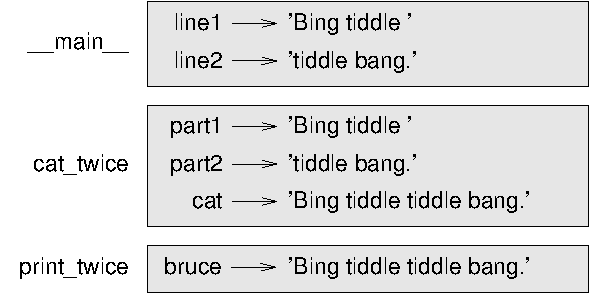
\includegraphics[scale=0.8]{../source/figs/stack.pdf}}
%🍁% \caption{Stack diagram.}
\caption{堆栈图。}
\label{fig.stack}
\end{figure}

%🍁% The frames are arranged in a stack that indicates which function
%🍁% called which, and so on.  In this example, \verb"print_twice"
%🍁% was called by \verb"cat_twice", and \verb"cat_twice" was called by
%🍁% \verb"__main__", which is a special name for the topmost frame.  When
%🍁% you create a variable outside of any function, it belongs to
%🍁% \verb"__main__".

这些线框排列成栈的形式,说明了哪个函数调用了哪个函数等信息。
在此例中,\li{print_twice} 被 \li{cat_twice} 调用,
\li{cat_twice} 又被 \li{__main__} 调用, \li{__main__} 是一个表示最上层栈帧的特殊名字。
当你在所有函数之外创建一个变量时,它就属于 \li{__main__}。

%🍁% Each parameter refers to the same value as its corresponding
%🍁% argument.  So, {\tt part1} has the same value as
%🍁% {\tt line1}, {\tt part2} has the same value as {\tt line2},
%🍁% and {\tt bruce} has the same value as {\tt cat}.

每个形参都指向其对应实参的值。
因此,\li{part1} 和 \li{line1} 的值相同, \li{part2} 和 \li{line2} 的值相同, \li{bruce} 和 \li{cat} 的值相同。

%🍁% If an error occurs during a function call, Python prints the
%🍁% name of the function, the name of the function that called
%🍁% it, and the name of the function that called {\em that}, all the
%🍁% way back to \verb"__main__".

如果函数调用时发生错误,Python会打印出错函数的名字以及调用它的函数的名字,
以及调用 *后面这个函数* 的函数的名字,一直追溯到 \li{__main__} 为止。

%🍁% For example, if you try to access {\tt cat} from within
%🍁% \verb"print_twice", you get a {\tt NameError}:

例如,如果你试图在 \li{print_twice} 里面访问 \li{cat} ,
你将获得一个 \li{NameError} :

%🍁% \begin{lstlisting}
%🍁% Traceback (innermost last):
%🍁%   File "test.py", line 13, in __main__
%🍁%     cat_twice(line1, line2)
%🍁%   File "test.py", line 5, in cat_twice
%🍁%     print_twice(cat)
%🍁%   File "test.py", line 9, in print_twice
%🍁%     print(cat)
%🍁% NameError: name 'cat' is not defined
%🍁% \end{lstlisting}
%🍁%

%🍁% This list of functions is called a {\bf traceback}.  It tells you what
%🍁% program file the error occurred in, and what line, and what functions
%🍁% were executing at the time.  It also shows the line of code that
%🍁% caused the error.

这个函数列表被称作 {\em 回溯} (traceback) 。
它告诉你发生错误的是哪个程序文件,错误在哪一行,以及当时在执行哪个函数。
它还会显示引起错误的那一行代码。
\index{traceback}

%🍁% The order of the functions in the traceback is the same as the
%🍁% order of the frames in the stack diagram.  The function that is
%🍁% currently running is at the bottom.

回溯中的函数顺序,与堆栈图中的函数顺序一致。出错时正在运行的那个函数则位于回溯信息的底部。


%
%%
% \section{Fruitful functions and void functions  |  有返回值函数和无返回值函数}
\section{有返回值函数和无返回值函数}
\index{fruitful function}  \index{void function}
\index{function, fruitful}  \index{function, void}
\index{有返回值函数}  \index{无返回值函数}
\index{函数function, 有返回值}  \index{函数, 无返回值}


%🍁% Some of the functions we have used, such as the math functions, return
%🍁% results; for lack of a better name, I call them {\bf fruitful
%🍁%   functions}.  Other functions, like \verb"print_twice", perform an
%🍁% action but don't return a value.  They are called {\bf void
%🍁%   functions}.

有一些我们之前用过的函数,例如数学函数,会返回结果;
由于没有更好的名字,我姑且叫它们 {\em 有返回值函数} (fruitful functions) 。
其它的函数,像 \li{print_twice} ,执行一个动作但是不返回任何值。
我称它们为 {\em 无返回值函数} (void functions) 。

%🍁% When you call a fruitful function, you almost always
%🍁% want to do something with the result; for example, you might
%🍁% assign it to a variable or use it as part of an expression:

当你调用一个有返回值函数时,你几乎总是想用返回的结果去做些什么;
例如,你可能将它赋值给一个变量,或者把它用在表达式里:

\begin{lstlisting}
x = math.cos(radians)
golden = (math.sqrt(5) + 1) / 2
\end{lstlisting}

%
%🍁% When you call a function in interactive mode, Python displays
%🍁% the result:

当你在交互模式下调用一个函数时,Python解释器会马上显示结果:

\begin{lstlisting}
>>> math.sqrt(5)
2.2360679774997898
\end{lstlisting}

%
%🍁% But in a script, if you call a fruitful function all by itself,
%🍁% the return value is lost forever!

但是在脚本中,如果你单单调用一个有返回值函数, 返回值就永远丢失了!

\begin{lstlisting}
math.sqrt(5)
\end{lstlisting}

%
%🍁% This script computes the square root of 5, but since it doesn't store
%🍁% or display the result, it is not very useful.

该脚本计算5的平方根,但是因为它没保存或者显示这个结果,
这个脚本并没多大用处。
\index{interactive mode}  \index{script mode}

%🍁% Void functions might display something on the screen or have some
%🍁% other effect, but they don't have a return value.  If you
%🍁% assign the result to a variable, you get a special value called
%🍁% {\tt None}.

无返回值函数可能在屏幕上打印输出结果,或者产生其它的影响,
但是它们并没有返回值。如果你试图将无返回值函数的结果赋给一个变量,
你会得到一个被称作 \li{None} 的特殊值。
\index{None special value}  \index{special value!None}

\begin{lstlisting}
>>> result = print_twice('Bing')
Bing
Bing
>>> print(result)
None
\end{lstlisting}

%
%🍁% The value {\tt None} is not the same as the string \verb"'None'".
%🍁% It is a special value that has its own type:

\li{None} 这个值和字符串 \li{'None'} 不同。 这是一个具有独立类型的特殊值:

\begin{lstlisting}
>>> print(type(None))
<class 'NoneType'>
\end{lstlisting}

%
%🍁% The functions we have written so far are all void.  We will start
%🍁% writing fruitful functions in a few chapters.

目前为止,我们写的函数都是无返回值函数。
我们将在几章之后开始编写有返回值函数。
\index{NoneType type}  \index{type!NoneType}


%
%%
% \section{Why functions?  |  为什么使用函数?}
\section{为什么使用函数?}
\index{function, reasons for}

%🍁% It may not be clear why it is worth the trouble to divide
%🍁% a program into functions.  There are several reasons:

%🍁% \begin{itemize}
%🍁%
%🍁% \item Creating a new function gives you an opportunity to name a group
%🍁% of statements, which makes your program easier to read and debug.
%🍁%
%🍁% \item Functions can make a program smaller by eliminating repetitive
%🍁% code.  Later, if you make a change, you only have
%🍁% to make it in one place.
%🍁%
%🍁% \item Dividing a long program into functions allows you to debug the
%🍁% parts one at a time and then assemble them into a working whole.
%🍁%
%🍁% \item Well-designed functions are often useful for many programs.
%🍁% Once you write and debug one, you can reuse it.
%🍁%
%🍁% \end{itemize}

你可能还不明白为什么值得将一个程序分解成多个函数。 原因包括以下几点:

\begin{itemize}

\item 创建一个新的函数可以让你给一组语句命名,这可以让你的程序更容易阅读和调试。

\item 通过消除重复的代码,函数精简了程序。 以后,如果你要做个变动,你只需在一处修改即可。

\item 将一个长程序分解为多个函数,可以让你一次调试一部分,然后再将它们组合为一个可行的整体。

\item 设计良好的函数经常对多个程序都有帮助。一旦你写出并调试好一个函数,你就可以重复使用它。

\end{itemize}


%
%%
% \section{Debugging  |  调试}
\section{调试}
\index{debug]}  \index{调试}

%🍁% One of the most important skills you will acquire is debugging.
%🍁% Although it can be frustrating, debugging is one of the most
%🍁% intellectually rich, challenging, and interesting parts of
%🍁% programming.

调试,是你能获得的最重要的技能之一。
虽然调试会让人沮丧,但却是编程过程中最富含智慧、挑战以及乐趣的一部分。
\index{experimental debugging}  \index{debugging!experimental}

%🍁% In some ways debugging is like detective work.  You are confronted
%🍁% with clues and you have to infer the processes and events that led
%🍁% to the results you see.

在某些方面,调试像是侦探工作。
你面对一些线索,必须推理出是什么进程 (processes) 和事件 (events)导致了你看到的结果。

%🍁% Debugging is also like an experimental science.  Once you have an idea
%🍁% about what is going wrong, you modify your program and try again.  If
%🍁% your hypothesis was correct, you can predict the result of the
%🍁% modification, and you take a step closer to a working program.  If
%🍁% your hypothesis was wrong, you have to come up with a new one.  As
%🍁% Sherlock Holmes pointed out, ``When you have eliminated the
%🍁% impossible, whatever remains, however improbable, must be the truth.''
%🍁% (A. Conan Doyle, {\em The Sign of Four})

调试也像是一门实验性科学。一旦你猜到大概哪里出错了,
你可以修改程序,再试一次。
如果你的假设是正确的,那么你就可以预测到修改的结果,并且离正常运行的程序又近了一步。
如果你的假设是错误的,你就不得不再提一个新的假设。
如夏洛克·福尔摩斯所指出的 ``当你排除了所有的不可能,无论剩下的是什么,
不管多么难以置信,一定就是真相。''(阿瑟·柯南·道尔,《{\em 四签名}》)
\index{Holmes, Sherlock}  \index{Doyle, Arthur Conan}

%🍁% For some people, programming and debugging are the same thing.  That
%🍁% is, programming is the process of gradually debugging a program until
%🍁% it does what you want.  The idea is that you should start with a
%🍁% working program and make small modifications,
%🍁% debugging them as you go.

对某些人来说,编程和调试是同一件事。
也就是说,编程是逐步调试一个程序,直到它满足了你期待的过程。
这意味着,你应该从一个能 {\em 正常运行} (working) 的程序开始,每次只做一些小改动,并同步进行调试。

%🍁% For example, Linux is an operating system that contains millions of
%🍁% lines of code, but it started out as a simple program Linus Torvalds
%🍁% used to explore the Intel 80386 chip.  According to Larry Greenfield,
%🍁% ``One of Linus's earlier projects was a program that would switch
%🍁% between printing AAAA and BBBB.  This later evolved to Linux.''
%🍁% ({\em The Linux Users' Guide} Beta Version 1).

举个例子,Linux是一个有着数百万行代码的操作系统 但是它一开始,只是Linus
Torvalds写的一个用于研究Intel 80386芯片的简单程序。 根据Larry
Greenfield的描述,“Linus的早期项目中,有一个能够交替打印AAAA和BBBB的程序。
这个程序后来演变为了Linux。”( {\em Linux用户手册} Beta 版本1)。
\index{Linux}


%
%%
% \section{Glossary  |  术语表}
\section{术语表}

\begin{description}

%🍁% \item[function:] A named sequence of statements that performs some
%🍁% useful operation.  Functions may or may not take arguments and may or
%🍁% may not produce a result.
%🍁% \index{function}

\item[函数 (function):] 执行某种有用运算的命名语句序列。函数可以接受形参,也可以不接受;可以返回一个结果,也可以不返回。
\index{function}  \index{函数}

%🍁% \item[function definition:]  A statement that creates a new function,
%🍁% specifying its name, parameters, and the statements it contains.
%🍁% \index{function definition}

\item[函数定义 (function definition:)] 创建一个新函数的语句,指定了函数名、形参以及所包含的语句。
\index{function definition}  \index{函数定义}

%🍁% \item[function object:]  A value created by a function definition.
%🍁% The name of the function is a variable that refers to a function
%🍁% object.
%🍁% \index{function definition}

\item[函数对象 (function object):] 函数定义所创建的一个值。函数名是一个指向函数对象的变量。
\index{function object}  \index{函数对象}

%🍁% \item[header:] The first line of a function definition.
%🍁% \index{header}

\item[函数头 (header):] 函数定义的第一行。
\index{header}  \index{函数头}

%🍁% \item[body:] The sequence of statements inside a function definition.
%🍁% \index{body}

\item[函数体 (body):] 函数定义内部的语句序列。
\index{body}  \index{函数体}

%🍁% \item[parameter:] A name used inside a function to refer to the value
%🍁% passed as an argument.
%🍁% \index{parameter}

\item[形参 (parameters):] 函数内部用于指向被传作实参的值的名字。
\index{parameter}  \index{形参}

%🍁% \item[function call:] A statement that runs a function. It
%🍁% consists of the function name followed by an argument list in
%🍁% parentheses.
%🍁% \index{function call}

\item[函数调用 (function call) :] 运行一个函数的语句。它包括了函数名,紧随其后的实参列表,实参用圆括号包围起来。
\index{function call}  \index{函数调用}

%🍁% \item[argument:]  A value provided to a function when the function is called. This value is assigned to the corresponding parameter in the function.

\item[实参 (argument) :] 函数调用时传给函数的值。这个值被赋给函数中相对应的形参。
\index{argument}  \index{实参}

%🍁% \item[local variable:]  A variable defined inside a function.  A local
%🍁% variable can only be used inside its function.

\item[局部变量 (local variable):] 函数内部定义的变量。局部变量只能在函数内部使用。
\index{local variable}  \index{局部变量}

%🍁% \item[return value:]  The result of a function.  If a function call
%🍁% is used as an expression, the return value is the value of
%🍁% the expression.

\item[返回值 (return value):] 函数执行的结果。如果函数调用被用作表达式,其返回值是这个表达式的值。
\index{return value}  \index{返回值}

%🍁% \item[fruitful function:] A function that returns a value.
%🍁% \index{fruitful function}

\item[有返回值函数 (fruitful function):] 会返回一个值的函数。
\index{fruitful function}  \index{有返回值函数}

%🍁% \item[void function:] A function that always returns {\tt None}.

\item[无返回值函数 (void function):]     总是返回None的函数。
\index{void function}  \index{无返回值函数}

%🍁% \item[{\tt None}:]  A special value returned by void functions.

\item[\tt None:] 无返回值函数返回的一个特殊值。
\index{None special value}  \index{special value!None}
\index{None 特殊值}  \index{特殊值!None}

%🍁% \item[module:] A file that contains a
%🍁% collection of related functions and other definitions.

\item[模块 (module):] 包含了一组相关函数及其他定义的的文件。
\index{module}

%🍁% \item[import statement:] A statement that reads a module file and creates
%🍁% a module object.

\item[导入语句 (import statement):] 读取一个模块文件,并创建一个模块对象的语句。
\index{import statement}  \index{statement!import}
\index{导入语句}  \index{语句!导入}

%🍁% \item[module object:] A value created by an {\tt import} statement
%🍁% that provides access to the values defined in a module.

\item[模块对象 (module object):] 导入语句创建的一个值, 可以让开发者访问模块内部定义的值。
\index{module}  \index{模块}

%🍁% \item[dot notation:]  The syntax for calling a function in another
%🍁% module by specifying the module name followed by a dot (period) and
%🍁% the function name.

\item[点标记法 (dot notation):] 调用另一个模块中函数的语法,需要指定模块名称,之后跟着一个点(句号)和函数名。
\index{dot notation}  \index{点标记法}

%🍁% \item[composition:] Using an expression as part of a larger expression,
%🍁% or a statement as part of a larger statement.

\item[组合 (composition):] 将一个表达式嵌入一个更长的表达式,或者是将一个语句嵌入一个更长语句的一部分。
\index{composition}  \index{组合}

%🍁% \item[flow of execution:]  The order statements run in.

\item[执行流程 (flow of execution):] 语句执行的顺序。
\index{flow of execution}  \index{执行流程}

%🍁% \item[stack diagram:]  A graphical representation of a stack of functions,
%🍁% their variables, and the values they refer to.

\item[堆栈图 (stack diagram):] 一种图形化表示堆栈的方法,堆栈中包括函数、函数的变量及其所指向的值。
\index{stack diagram}  \index{堆栈图}

%🍁% \item[frame:]  A box in a stack diagram that represents a function call.
%🍁% It contains the local variables and parameters of the function.

\item[栈帧 (frame) :] 堆栈图中一个栈帧,代表一个函数调用。其中包含了函数的局部变量和形参。
\index{function frame}  \index{frame}
\index{函数栈帧}  \index{栈帧}

%🍁% \item[traceback:]  A list of the functions that are executing,
%🍁% printed when an exception occurs.

\item[回溯 (traceback) :] 当出现异常时,解释器打印出的出错时正在执行的函数列表。
\index{traceback}  \index{回溯}

\end{description}


%
%%
% \section{Exercises  |  练习}
\section{练习}

\begin{exercise}
\index{len function}  \index{function!len}

%🍁% Write a function named \verb"right_justify" that takes a string
%🍁% named {\tt s} as a parameter and prints the string with enough
%🍁% leading spaces so that the last letter of the string is in column 70
%🍁% of the display.

编写一个名为 {\em \li{right_justify}} 的函数,函数接受一个名为 {\em \li{s}}的字符串作为形参, 并在打印足够多的前导空格 {\em (leading space)} 之后打印这个字符串,使得字符串的最后一个字母位于显示屏的第 {\em 70} 列。

\begin{em}
\begin{lstlisting}
>>> right_justify('monty')
                                                                 monty
\end{lstlisting}
\end{em}

%🍁% Hint: Use string concatenation and repetition.  Also,
%🍁% Python provides a built-in function called {\tt len} that
%🍁% returns the length of a string, so the value of \verb"len('monty')" is 5.

提示:使用字符串拼接 {\em (string concatenation)} 和重复。 另外,{\em Python}提供了一个名叫 {\em \li{len}} 的内建函数,可以返回一个字符串的长度,因此 {\em \li{len('allen')}} 的值是 {\em 5}。

\end{exercise}


\begin{exercise}
\index{function object}  \index{object!function}

%🍁% A function object is a value you can assign to a variable
%🍁% or pass as an argument.  For example, \verb"do_twice" is a function
%🍁% that takes a function object as an argument and calls it twice:

函数对象是一个可以赋值给变量的值,也可以作为实参传递。例如,
{\em \li{do_twice}} 函数接受函数对象作为实参,并调用这个函数对象两次:

\begin{em}
\begin{lstlisting}
def do_twice(f):
    f()
    f()
\end{lstlisting}
\end{em}
%🍁% Here's an example that uses \verb"do_twice" to call a function
%🍁% named \verb"print_spam" twice.


下面这个示例使用 {\em \li{do_twice}} 来调用名为 {\em \li{print_spam}} 的函数两次。

\begin{em}
\begin{lstlisting}
def print_spam():
    print('spam')

do_twice(print_spam)
\end{lstlisting}
\end{em}

%🍁% \begin{enumerate}
%🍁%
%🍁% \item Type this example into a script and test it.
%🍁%
%🍁% \item Modify \verb"do_twice" so that it takes two arguments, a
%🍁% function object and a value, and calls the function twice,
%🍁% passing the value as an argument.
%🍁%
%🍁% \item Copy the definition of
%🍁% \verb"print_twice" from earlier in this chapter to your script.
%🍁%
%🍁% \item Use the modified version of \verb"do_twice" to call
%🍁% \verb"print_twice" twice, passing \verb"'spam'" as an argument.
%🍁%
%🍁% \item Define a new function called
%🍁% \verb"do_four" that takes a function object and a value
%🍁% and calls the function four times, passing the value
%🍁% as a parameter.  There should be only
%🍁% two statements in the body of this function, not four.
%🍁%
%🍁% \end{enumerate}

\begin{enumerate}

\item 将这个示例写入脚本,并测试。

\item 修改 {\em \li{do_twice}},使其接受两个实参,一个是函数对象,另一个是值。
   然后调用这一函数对象两次,将那个值传递给函数对象作为实参。

\item 从本章前面一些的示例中,将 {\em \li{print_twice}} 函数的定义复制到脚本中。

\item 使用修改过的 {\em \li{do_twice}} ,调用 {\em \li{print_twice}} 两次,将 {\em \li{spam}} 传递给它作为实参。

\item 定义一个名为 {\em \li{do_four}} 的新函数,其接受一个函数对象和一个值作为实参。 调用这个函数对象四次,将那个值作为形参传递给它。 函数体中应该只有两条语句,而不是四条。

\end{enumerate}

%🍁% Solution: \href{http://thinkpython2.com/code/do_four.py}{Solution}.

\href{http://thinkpython2.com/code/do_four.py}{参考答案}

\end{exercise}



\begin{exercise}

%🍁% Note: This exercise should be done using only the statements and other features we have learned so far.

注意:请使用我们目前学过的语句和特性来完成本题。

%🍁% \begin{enumerate}

%🍁% \item Write a function that draws a grid like the following:
%🍁% \index{grid}

%🍁% \begin{lstlisting}
%🍁% + - - - - + - - - - +
%🍁% |         |         |
%🍁% |         |         |
%🍁% |         |         |
%🍁% |         |         |
%🍁% + - - - - + - - - - +
%🍁% |         |         |
%🍁% |         |         |
%🍁% |         |         |
%🍁% |         |         |
%🍁% + - - - - + - - - - +
%🍁% \end{lstlisting}
%🍁% %
%🍁% Hint: to print more than one value on a line, you can print
%🍁% a comma-separated sequence of values:
%🍁%
%🍁% \begin{lstlisting}
%🍁% print('+', '-')
%🍁% \end{lstlisting}
%🍁% %
%🍁% By default, {\tt print} advances to the next line, but you
%🍁% can override that behavior and put a space at the end, like this:
%🍁%
%🍁% \begin{lstlisting}
%🍁% print('+', end=' ')
%🍁% print('-')
%🍁% \end{lstlisting}
%🍁% %
%🍁% The output of these statements is \verb"'+ -'".
%🍁%
%🍁% A {\tt print} statement with no argument ends the current line and
%🍁% goes to the next line.
%🍁%
%🍁% \item Write a function that draws a similar grid
%🍁% with four rows and four columns.
%🍁%
%🍁% \end{enumerate}


\begin{enumerate}

\item 编写一个能画出如下网格 {\em (grid)} 的函数:
\index{grid}

\begin{em}
\begin{lstlisting}
+ - - - - + - - - - +
|         |         |
|         |         |
|         |         |
|         |         |
+ - - - - + - - - - +
|         |         |
|         |         |
|         |         |
|         |         |
+ - - - - + - - - - +
\end{lstlisting}
\end{em}

%
提示:你可以使用一个用逗号分隔的值序列,在一行中打印出多个值:

\begin{em}
\begin{lstlisting}
print('+', '-')
\end{lstlisting}
\end{em}

%
{\em \li{print}} 函数默认会自动换行,但是你可以阻止这个行为,只需要像下面这样将行结尾变成一个空格:

\begin{em}
\begin{lstlisting}
print('+', end=' ')
print('-')
\end{lstlisting}
\end{em}

%
这两个语句的输出结果是 {\em \li{+ -'}}。

一个没有传入实参的 {\em \li{print}} 语句会结束当前行,跳到下一行。

\item 编写一个能够画出四行四列的类似网格的函数。

\end{enumerate}


\href{http://thinkpython2.com/code/grid.py}{参考答案}

%🍁%  Credit: This exercise is based on an exercise in Oualline, {\em
%🍁%      Practical C Programming, Third Edition}, O'Reilly Media, 1997.

致谢:这个习题基于 {\em Practical C Programming, Third
Edition} 一书中的习题改编,该书由 {\em O’Reilly} 出版社于{\em 1997}年出版。

\end{exercise}

